%!TEX root = ../thesis.tex

\section{Encoding \& Decoding Data Simulation}
\label{sec:enc-dec-theory}

	All of the coding schemes as discussed in \autoref{sec:CDMA} are designed for wireless transceivers.
	Meaning they send a radio wave through the air which is encoded with that particular code sequence.
	That radio wave is an analog signal and can vary between $+1$ and $-1$ symbols.
	But the VLC enabled LEDs cannot send such signals.
	They can only be turned on or off, thus encoding only $0$ and $1$ symbols.
	Those symbols correspond to a current draw of the LED which is measured by an ADC for example.
	To experiment with the encoding and decoding process and obstacles without the need for hardware, we use Matlab to simulate the process.

	\subsection{Walsh-Hadamard Sequences}

		%about radio dec. and bin. enc. proof etc...
		The way the Walsh-Hadamard sequences work with encoding and decoding with for example the link from a base-station to a mobile device of a CDMA application, is that the sequence of $+1$ and $-1$ symbols gets multiplied with the encoded data. 
		Say for example that we have a Hadamard matrix of rank $8$ as can be seen in \autoref{matrix:h8} which is created by using \autoref{eq:hadamard-matrix-creation}.
		And we select a random code to encode our data with, which corresponds to a row of this matrix.
		We also assume that our data is binary, consisting of 0s and 1s. 
		Our last assumption is that is we want to encode a $0$ we use the code itself and if we want to encode a $1$ we use the inverse of the code, i.e. $-1 \times$ the code.
		That describes the encoding process. 
		The decoding process involves the calculation of the correlation of the received signal with a code sequence for which we want to know if there is information embedded in the received signal and if so, what might that information be.

			\begin{equation}
				H_8 = 
				\begin{bmatrix*}[r] 
					H_4 & H_4 \\ 
					H_4 & -H_4 
				\end{bmatrix*}
				%=
				%\begin{bmatrix*}[r] 
				%	H_2 & H_2   & H_2 & H_2   \\
				%	H_2 & -H_2  & H_2 & -H_2  \\
				%	H_2 & H_2   & -H_2 & -H_2 \\
				%	H_2 & -H_2  & -H_2 & H_2  \\
				%\end{bmatrix*}
				=
				\dotsc
				=
				\begin{bmatrix*}[r]
					1	&	 1	&	 1	&	 1	&	 1	&	 1	&	 1	&	 1 \\
					1	&	-1	&	 1	&	-1	&	 1	&	-1	&	 1	&	-1 \\
					1	&	 1	&	-1	&	-1	&	 1	&	 1	&	-1	&	-1 \\
					1	&	-1	&	-1	&	 1	&	 1	&	-1	&	-1	&	 1 \\
					1	&	 1	&	 1	&	 1	&	-1	&	-1	&	-1	&	-1 \\
					1	&	-1	&	 1	&	-1	&	-1	&	 1	&	-1	&	 1 \\
					1	&	 1	&	-1	&	-1	&	-1	&	-1	&	 1	&	 1 \\
					1	&	-1	&	-1	&	 1	&	-1	&	 1	&	 1	&	-1 
				\end{bmatrix*}
				\label{matrix:h8}
			\end{equation}

		Since the autocorrelation of Walsh-Hadamard sequences do not allow to find the beginning of a code, see \autoref{fig:autocorr-hadamard}, we will only consider the synchronized situation, for which these codes are also used in practice, so $\tau = 0$.
		Say we have a code $c_i(t)$ and we want to encode a $0$ with this code and send that as a signal for our receiver to receive.
		The receiver will receive this signal $s(t)$ assuming a perfect channel, the decoding process can be seen below.

		%Want something different than proof, but dont know how/what

		\begin{proof}
			Let $s(t)$ be the received signal which encodes a 0 for code: $c_i(t)$.\\
			And let $c_i(t)$ be the code for which we want to check if there is information there. \\

			\begin{align*}
				R(\tau)_{xy} = \displaystyle\sum_{t = 0} ^ {L - 1} x(t) \times y(t + \tau)	\tag{See \autoref{eq:correlation}}
				\\ \tau = 0,\ x = s(t),\ y = c_i(t)	
				\\ R(0)_{sc_{i}} = \displaystyle\sum_{t = 0} ^ {L - 1} s(t) \times c_i(t)	
				\\ s(t) = c_i(t)															
				\\ R(0)_{sc_{i}} = \displaystyle\sum_{t = 0} ^ {L - 1} c_i(t) \times c_i(t) = L
			\end{align*}

		\end{proof}

		We can also state what the result will be when we decode a $1$ with a code $c_i(t)$, see below:

		\begin{proof}
			Let $s(t)$ be the received signal which encodes a 1 for code: $c_i(t)$.\\
			And let $c_i(t)$ be the code for which we want to check if there is information there. \\

			\begin{align*}
				R(\tau)_{xy} = \displaystyle\sum_{t = 0} ^ {L - 1} x(t) \times y(t + \tau)	\tag{See \autoref{eq:correlation}}
				\\ \tau = 0,\ x = s(t),\ y = c_i(t)	
				\\ R(0)_{sc_{i}} = \displaystyle\sum_{t = 0} ^ {L - 1} s(t) \times c_i(t)	
				\\ s(t) = -1 \times c_i(t)															
				\\ R(0)_{sc_{i}} = \displaystyle\sum_{t = 0} ^ {L - 1} -1 \times c_i(t) \times c_i(t)
				\\ &= -1 \times \displaystyle\sum_{t = 0} ^ {L - 1} c_i(t) \times c_i(t) = -1 \times L
			\end{align*}

		\end{proof}

		This two statement state that if we encode a data bit with code $c_i$ and that is the only information received by the receiver, we either get the maximum positive correlation, i.e. $L$ or we get the maximum negative correlation, i.e. $-L$.
		If we would have received a signal consisting of only zeros the correlation would also be zero.

		Next let us look at what happens when we try to decode information with a different code than the code which was used to encode information with. In that case we also get a correlation of zero, see below. This is per definition the case since we are using Walsh-Hadamard codes which are orthogonal to each other when they are synchronized.

		\begin{proof}
			Let $s(t)$ be the received signal which encodes a data bit for code: $c_i(t)$.\\
			And let $c_j(t)$ be the code for which we want to check if there is information there. \\

			\begin{align*}
				R(\tau)_{xy} = \displaystyle\sum_{t = 0} ^ {L - 1} x(t) \times y(t + \tau)	\tag{See \autoref{eq:correlation}}
				\\ \tau = 0,\ x = s(t),\ y = c_j(t)	
				\\ R(0)_{sc_{i}} = \displaystyle\sum_{t = 0} ^ {L - 1} s(t) \times c_j(t)	
				\\ s(t) = c_i(t)															
				\\ R(0)_{sc_{i}} = \displaystyle\sum_{t = 0} ^ {L - 1} c_i(t) \times c_j(t) = 0
			\end{align*}

		\end{proof}

		Finally we look at the decoding process for when the received signal consists of several encoded signals, see below. 
		Because all the codes in Walsh-Hadamard sequences are orthogonal to each other they produce no MAI and so there can be as many codes superimposed on each other and still a correct decoding can take place. 


		\begin{proof}
			Let $s(t)$ be the received signal which encodes data for several codes: $c_i(t)$, $c_j(t)$, $c_k(t)$ and $c_l(t)$.\\
			And let $c_i(t)$ be the code for which we want to check if there is information there. \\

			\begin{align*}
				R(\tau)_{xy} = \displaystyle\sum_{t = 0} ^ {L - 1} x(t) \times y(t + \tau)	\tag{See \autoref{eq:correlation}}
				\\ \tau = 0,\ x = s(t),\ y = c_i(t)	
				\\ R(0)_{sc_{i}} = \displaystyle\sum_{t = 0} ^ {L - 1} s(t) \times c_i(t)	
				\\ s(t) = c_i(t) + c_j(t) + c_k(t) + c_l(t)															
				\\ R(0)_{sc_{i}} = \displaystyle\sum_{t = 0} ^ {L - 1} \{ c_i(t) + c_j(t) + c_k(t) + c_l(t) \} \times c_i(t)
				\\ R(0)_{sc_{i}} = \displaystyle\sum_{t = 0} ^ {L - 1} c_i(t) \times c_i(t) + c_j(t) \times c_i(t) + c_k(t) \times c_i(t) + c_l(t) \times c_i(t)
				\\ = L + 0 + 0 + 0 = L
			\end{align*}

		\end{proof}

		But as stated in \autoref{sec:enc-dec-theory} the VLC enabled LEDs cannot send $+1$ and $-1$ symbols of data, they can only be in an on or off state.
		This means that the code that is being used for encoding must be mapped to zeros and ones.
		Let us assume that a $+1$ symbol maps to an off state, i.e. $0$ and that a $-1$ symbol maps to an on state, i.e. $1$.
		We can summarize that in \autoref{eq:radio-to-bin}, where $r$ denotes the $+1$ or $-1$ symbols and the outcome $b$ will be our binary value, i.e. $0$ or $1$.

		\begin{equation}
			b = \frac{1 - r}{2}
			\label{eq:radio-to-bin}
		\end{equation}

		Because we are now using the binary values as code, we can no longer use multiply to encode our binary information.
		Instead, we must use the XOR function.
		Now let us see what happens when we try to decode information that has been encoded using on-off keying (OOK), below is stated what happens when both data bits are encoded.

		\begin{proof}
			Let $s(t)$ be the received signal which encodes a 0 for code: $c^b_i(t)$, where $c^b_i(t)$ is binary valued, i.e. $0$ or $1$ \\
			And let $c^r_i(t)$ be the code for which we want to check if there is information there, where $c^r_i(t)$ uses the traditional values $-1$ and $+1$ \\

			\begin{align*}
				R(\tau)_{xy} = \displaystyle\sum_{t = 0} ^ {L - 1} x(t) \times y(t + \tau)	\tag{See \autoref{eq:correlation}}
				\\ \tau = 0,\ x = s(t),\ y = c^r_i(t)	
				\\ R(0)_{sc^r_{i}} = \displaystyle\sum_{t = 0} ^ {L - 1} s(t) \times c^r_i(t)	
				\\ s(t) = \forall t \in \{ 0, 1, 2, \dotsc, L - 1 \} \ \ 0(t) \oplus c^b_i(t) = c^b_i(t) \tag{Where $0(t) = 0 \ \forall t$ }										
				\\ R(0)_{sc^r_{i}} = \displaystyle\sum_{t = 0} ^ {L - 1} c^b_i(t) \times c^r_i(t)
				\\ = \displaystyle\sum_{t = 0} ^ {L - 1} \frac{1 - c^r_i(t)}{2} \times c^r_i(t) \tag{Via \autoref{eq:radio-to-bin}}
				\\ = \frac{1}{2} \times \displaystyle\sum_{t = 0} ^ {L - 1} c^r_i(t) - c^r_i(t) \times c^r_i(t)
				\\ = \frac{1}{2} \times \displaystyle\sum_{t = 0} ^ {L - 1} c^r_i(t) - \frac{1}{2} \times \displaystyle\sum_{t = 0} ^ {L - 1} c^r_i(t) \times c^r_i(t)
				\\ = 0 - \frac{1}{2} \times \displaystyle\sum_{t = 0} ^ {L - 1} c^r_i(t) \times c^r_i(t) \tag{Balance property}
				\\ = - \frac{1}{2} \times L
			\end{align*}

		\end{proof}

		\begin{proof}
			Let $s(t)$ be the received signal which encodes a 1 for code: $c^b_i(t)$, where $c^b_i(t)$ is binary valued, i.e. $0$ or $1$ \\
			And let $c^r_i(t)$ be the code for which we want to check if there is information there, where $c^r_i(t)$ uses the traditional values $-1$ and $+1$ \\

			\begin{align*}
				R(\tau)_{xy} = \displaystyle\sum_{t = 0} ^ {L - 1} x(t) \times y(t + \tau)	\tag{See \autoref{eq:correlation}}
				\\ \tau = 0,\ x = s(t),\ y = c^r_i(t)	
				\\ R(0)_{sc^r_{i}} = \displaystyle\sum_{t = 0} ^ {L - 1} s(t) \times c^r_i(t)	
				\\ s(t) = \forall t \in \{ 0, 1, 2, \dotsc, L - 1 \} \ \ 1(t) \oplus c^b_i(t) = 1 - c^b_i(t) \tag{Where $1(t) = 1 \ \forall t$ }
				\\ R(0)_{sc^r_{i}} = \displaystyle\sum_{t = 0} ^ {L - 1} (1 - c^b_i(t)) \times c^r_i(t)
				\\ = \displaystyle\sum_{t = 0} ^ {L - 1} (1 - \frac{1 - c^r_i(t)}{2}) \times c^r_i(t) \tag{Via \autoref{eq:radio-to-bin}}
				\\ = \displaystyle\sum_{t = 0} ^ {L - 1} \frac{1 + c^r_i(t)}{2} \times c^r_i(t)
				\\ = \frac{1}{2} \times \displaystyle\sum_{t = 0} ^ {L - 1} c^r_i(t) + c^r_i(t) \times c^r_i(t)
				\\ = \frac{1}{2} \times \displaystyle\sum_{t = 0} ^ {L - 1} c^r_i(t) + \frac{1}{2} \times \displaystyle\sum_{t = 0} ^ {L - 1} c^r_i(t) \times c^r_i(t)
				\\ = 0 + \frac{1}{2} \times \displaystyle\sum_{t = 0} ^ {L - 1} c^r_i(t) \times c^r_i(t) \tag{Balance property}
				\\ = \frac{1}{2} \times L
			\end{align*}

		\end{proof}

		The case for when there is no data encoded for this particular code:

		\begin{proof}
			Let $s(t)$ be the received signal which encodes data for code: $c^b_i(t)$, where $c^b_i(t)$ is binary valued, i.e. $0$ or $1$ \\
			And let $c^r_j(t)$ be the code for which we want to check if there is information there, where $c^r_j(t)$ uses the traditional values $-1$ and $+1$ \\

			\begin{align*}
				R(\tau)_{xy} = \displaystyle\sum_{t = 0} ^ {L - 1} x(t) \times y(t + \tau)	\tag{See \autoref{eq:correlation}}
				\\ \tau = 0,\ x = s(t),\ y = c^r_j(t)	
				\\ R(0)_{sc^r_{i}} = \displaystyle\sum_{t = 0} ^ {L - 1} s(t) \times c^r_j(t)	
				\\ s(t) = c^b_i(t)										
				\\ R(0)_{sc^r_{i}} = \displaystyle\sum_{t = 0} ^ {L - 1} c^b_i(t) \times c^r_j(t)
				\\ = \displaystyle\sum_{t = 0} ^ {L - 1} \frac{1 - c^r_i(t)}{2} \times c^r_j(t) \tag{Via \autoref{eq:radio-to-bin}}
				\\ = \frac{1}{2} \times \displaystyle\sum_{t = 0} ^ {L - 1} c^r_j(t) - c^r_i(t) \times c^r_j(t)
				\\ = \frac{1}{2} \times \displaystyle\sum_{t = 0} ^ {L - 1} c^r_j(t) - \frac{1}{2} \times \displaystyle\sum_{t = 0} ^ {L - 1} c^r_i(t) \times c^r_j(t)
				\\ = 0 - \frac{1}{2} \times \displaystyle\sum_{t = 0} ^ {L - 1} c^r_i(t) \times c^r_i(t) \tag{Balance property}
				\\ = 0 + 0 = 0\tag{Because the codes are orthogonal.}
			\end{align*}

		\end{proof}

		Finally the case for when there are multiple signals:


		\begin{proof}
			Let $s(t)$ be the received signal which encodes data for several codes: $c^b_i(t)$, $c^b_j(t)$, $c^b_k(t)$ and $c^b_l(t)$, where $c^b_i(t)$ is binary valued, i.e. $0$ or $1$\\
			And let $c^r_i(t)$ be the code for which we want to check if there is information there, where $c^r_i(t)$ uses the traditional values $-1$ and $+1$ \\

			\begin{align*}
				R(\tau)_{xy} = \displaystyle\sum_{t = 0} ^ {L - 1} x(t) \times y(t + \tau)	\tag{See \autoref{eq:correlation}}
				\\ \tau = 0,\ x = s(t),\ y = c^r_i(t)	
				\\ R(0)_{sc^r_{i}} = \displaystyle\sum_{t = 0} ^ {L - 1} s(t) \times c^r_i(t)	
				\\ s(t) = c^b_i(t) + c^b_j(t) + c^b_k(t) + c^b_l(t)															
				\\ R(0)_{sc^r_{i}} = \displaystyle\sum_{t = 0} ^ {L - 1} \{ c^b_i(t) + c^b_j(t) + c^b_k(t) + c^b_l(t) \} \times c^r_i(t)
				\\ R(0)_{sc^r_{i}} = \displaystyle\sum_{t = 0} ^ {L - 1} c^b_i(t) \times c^r_i(t) + c^b_j(t) \times c^r_i(t) + c^b_k(t) \times c^r_i(t) + c^b_l(t) \times c^r_i(t)
				\\ = \frac{1}{2} \times L + 0 + 0 + 0 = \frac{1}{2} \times L \tag{See above proofs}
			\end{align*}

		\end{proof}




		As we can see the correlation is for both data bits and when there is no information encoded, exactly $-\frac{1}{2}$ times as large as when dealing only with $+1$ and $-1$ symboled codes. 
		It also works for when there are multiple streams of encoded information present in the signal received.
		A summary is available, see \autoref{tbl:correlation-levels}.

		\begin{table}[h!]
			\centering
			
			\begin{tabular}{| l | l |}
				\hline
				Method												& Correlation \\ \hline \hline
				Encoding a 0 and decoding with only one transmitter & $-\frac{1}{2} \times L$  \\ \hline
				Encoding a 1 and decoding with only one transmitter & $ \frac{1}{2} \times L$   \\ \hline
				Encoding a 0 and decoding with a different code, with only one transmitter & 0  \\ \hline
				Encoding a 0 and decoding with multiple transmitters & $-\frac{1}{2} \times L$ \\ \hline
			\end{tabular}
			\caption{Table containing summary of correlation levels.}
			\label{tbl:correlation-levels}
		\end{table}









		We can also choose to encode and decode with the binary valued codes only, so only use values with $0$ and $1$. 


		\begin{proof}
			Let $s(t)$ be the received signal which encodes a 0 for code: $c^b_i(t)$, where $c^b_i(t)$ is binary valued, i.e. $0$ or $1$ \\
			And let $c^b_i(t)$ be the code for which we want to check if there is information there, where $c^b_i(t)$ is binary valued, i.e. $0$ or $1$ \\

			\begin{align*}
				R(\tau)_{xy} = \displaystyle\sum_{t = 0} ^ {L - 1} x(t) \times y(t + \tau)	\tag{See \autoref{eq:correlation}}
				\\ \tau = 0,\ x = s(t),\ y = c^b_i(t)	
				\\ R(0)_{sc^b_{i}} = \displaystyle\sum_{t = 0} ^ {L - 1} s(t) \times c^b_i(t)	
				\\ s(t) = \forall t \in \{ 0, 1, 2, \dotsc, L - 1 \} \ \ 0(t) \oplus c^b_i(t) = c^b_i(t) \tag{Where $0(t) = 0 \ \forall t$ }
				\\ R(0)_{sc^b_{i}} = \displaystyle\sum_{t = 0} ^ {L - 1} c^b_i(t) \times c^b_i(t)
				\\ = \displaystyle\sum_{t = 0} ^ {L - 1} \frac{1 - c^r_i(t)}{2} \times \frac{1 - c^r_i(t)}{2} \tag{Via \autoref{eq:radio-to-bin}}
				\\ = \frac{1}{4} \times \displaystyle\sum_{t = 0} ^ {L - 1} 1 - 2 \times c^r_i(t) + c^r_i(t) \times c^r_i(t)
				\\ = \frac{1}{4} \times \displaystyle\sum_{t = 0} ^ {L - 1} 1 - \frac{1}{2} \times \displaystyle\sum_{t = 0} ^ {L - 1} c^r_i(t) + \frac{1}{4} \times \displaystyle\sum_{t = 0} ^ {L - 1} c^r_i(t) \times c^r_i(t)
				\\ = \frac{1}{4} \times L - 0 + \frac{1}{4} \times L = \frac{1}{2} \times L
			\end{align*}

		\end{proof}


		\begin{proof}
			Let $s(t)$ be the received signal which encodes a 1 for code: $c^b_i(t)$, where $c^b_i(t)$ is binary valued, i.e. $0$ or $1$ \\
			And let $c^b_i(t)$ be the code for which we want to check if there is information there, where $c^b_i(t)$ is binary valued, i.e. $0$ or $1$ \\

			\begin{align*}
				R(\tau)_{xy} = \displaystyle\sum_{t = 0} ^ {L - 1} x(t) \times y(t + \tau)	\tag{See \autoref{eq:correlation}}
				\\ \tau = 0,\ x = s(t),\ y = c^b_i(t)	
				\\ R(0)_{sc^b_{i}} = \displaystyle\sum_{t = 0} ^ {L - 1} s(t) \times c^b_i(t)	
				\\ s(t) = \forall t \in \{ 0, 1, 2, \dotsc, L - 1 \} \ \ 1(t) \oplus c^b_i(t) = 1 - c^b_i(t) \tag{Where $1(t) = 1 \ \forall t$ }
				\\ R(0)_{sc^b_{i}} = \displaystyle\sum_{t = 0} ^ {L - 1} (1 - c^b_i(t)) \times c^b_i(t)
				\\ = \displaystyle\sum_{t = 0} ^ {L - 1} (1 - \frac{1 - c^r_i(t)}{2}) \times \frac{1 - c^r_i(t)}{2} \tag{Via \autoref{eq:radio-to-bin}}
				\\ = \displaystyle\sum_{t = 0} ^ {L - 1} \frac{1 + c^r_i(t)}{2} \times \frac{1 - c^r_i(t)}{2}
				\\ = \frac{1}{4} \times \displaystyle\sum_{t = 0} ^ {L - 1} 1 - c^r_i(t) \times c^r_i(t)
				\\ = \frac{1}{4} \times \displaystyle\sum_{t = 0} ^ {L - 1} 1 - \frac{1}{4} \times \displaystyle\sum_{t = 0} ^ {L - 1} c^r_i(t) \times c^r_i(t)
				\\ = \frac{1}{4} \times L - \frac{1}{4} \times \displaystyle\sum_{t = 0} ^ {L - 1} c^r_i(t) \times c^r_i(t)
				\\ = \frac{1}{4} \times L - \frac{1}{4} \times L = 0
			\end{align*}

		\end{proof}

		\begin{proof}
			Let $s(t)$ be the received signal which encodes a 0 for code: $c^b_i(t)$, where $c^b_i(t)$ is binary valued, i.e. $0$ or $1$ \\
			And let $c^b_j(t)$ be the code for which we want to check if there is information there, where $c^b_i(t)$ is binary valued, i.e. $0$ or $1$ \\

			\begin{align*}
				R(\tau)_{xy} = \displaystyle\sum_{t = 0} ^ {L - 1} x(t) \times y(t + \tau)	\tag{See \autoref{eq:correlation}}
				\\ \tau = 0,\ x = s(t),\ y = c^b_j(t)	
				\\ R(0)_{sc^b_{j}} = \displaystyle\sum_{t = 0} ^ {L - 1} s(t) \times c^b_j(t)	
				\\ s(t) = \forall t \in \{ 0, 1, 2, \dotsc, L - 1 \} \ \ 0(t) \oplus c^b_i(t) = c^b_i(t) \tag{Where $0(t) = 0 \ \forall t$ }
				\\ R(0)_{sc^b_{j}} = \displaystyle\sum_{t = 0} ^ {L - 1} c^b_i(t) \times c^b_j(t)
				\\ = \displaystyle\sum_{t = 0} ^ {L - 1} \frac{1 - c^r_i(t)}{2} \times \frac{1 - c^r_j(t)}{2} \tag{Via \autoref{eq:radio-to-bin}}
				\\ = \frac{1}{4} \times \displaystyle\sum_{t = 0} ^ {L - 1} 1 - c^r_i(t) - c^r_j(t) + c^r_i(t) \times c^r_j(t)
				\\ = \frac{1}{4} \times \displaystyle\sum_{t = 0} ^ {L - 1} 1 - \frac{1}{4} \times \displaystyle\sum_{t = 0} ^ {L - 1} c^r_i(t) - \frac{1}{4} \times \displaystyle\sum_{t = 0} ^ {L - 1} c^r_j(t) + \frac{1}{4} \times \displaystyle\sum_{t = 0} ^ {L - 1} c^r_i(t) \times c^r_j(t) 
				\\ = \frac{1}{4} \times L - 0 - 0 + 0 = \frac{1}{4} \times L
			\end{align*}

		\end{proof}

		\begin{proof}
			Let $s(t)$ be the received signal which encodes data for codes: $c^b_j(t)$, $c^b_l(t)$, where $c^b_j(t)$ is binary valued, i.e. $0$ or $1$\\
			And let $c^b_i(t)$ be the code for which we want to check if there is information there, where $c^b_i(t)$ is binary valued, i.e. $0$ or $1$ \\

			\begin{align*}
				R(\tau)_{xy} = \displaystyle\sum_{t = 0} ^ {L - 1} x(t) \times y(t + \tau)	\tag{See \autoref{eq:correlation}}
				\\ \tau = 0,\ x = s(t),\ y = c^b_i(t)	
				\\ R(0)_{sc^b_{i}} = \displaystyle\sum_{t = 0} ^ {L - 1} s(t) \times c^r_i(t)	
				\\ s(t) = c^b_j(t) + c^b_l(t)														
				\\ R(0)_{sc^b_{i}} = \displaystyle\sum_{t = 0} ^ {L - 1} \{ c^b_j(t) + c^b_l(t) \} \times c^b_i(t)
				\\ R(0)_{sc^b_{i}} = \displaystyle\sum_{t = 0} ^ {L - 1} c^b_j(t) \times c^b_i(t) + c^b_l(t) \times c^b_i(t)
				\\ = \frac{1}{4} \times L + \frac{1}{4} \times L = \frac{1}{2} \times L \tag{See above proofs}
			\end{align*}

		\end{proof}



		\begin{table}[h!]
			\centering
			
			\begin{tabular}{| l | l |}
				\hline
				Method												& Correlation \\ \hline \hline
				Encoding a 0 and decoding with only one transmitter 							& $\frac{1}{2} \times L$  \\ \hline
				Encoding a 1 and decoding with only one transmitter 							& $ 0 $   \\ \hline
				Encoding a 0 and decoding with a different code, with only one transmitter 		& $\frac{1}{4} \times L$  \\ \hline
				Encoding a 0 and decoding with a different code, with two transmitters			& $\frac{1}{2} \times L$  \\ \hline
			\end{tabular}
			\caption{Table containing summary of correlation levels.}
			\label{tbl:correlation-levels-bin}
		\end{table}

		As we can see from the summary in \autoref{tbl:correlation-levels-bin}, the correlation levels for decoding one transmitter with the correct code, is the same as the correlation level from decoding with a code that was not encoded.
		This forms a problem as we cannot distinguish correctly these cases.
		And as a result we cannot use this decoding scheme. 


		In the synchronous case, for which these codes are also used in practice, we can correctly encode and subsequently decode information. 
		Without experiencing false-positives and without false-negatives.
		There can also be as much transmitters transmitting concurrently without MAI as there are codes available, because the codes are orthogonal.
		The only downside to this scheme is that all of the transmitter have to work together, they have to transmit synchronously.





	\subsection{PN Sequences}

		As we know from \autoref{sec:theory-pn}, there is no particular bound on the cross-correlation between two or more PN sequences.
		This means that they will have MAI and that there is a limit on how many transmitters can transmit at the same time, with the the receiver still able to correctly decode the information without experiencing false-positives and/or false-negatives.

		Since there is no particular bound on the cross-correlation with PN sequences from the same length, they need to be calculated.
		The calculated results can be seen in \autoref{tbl:correlation-pn-families}.


		\begin{table}
			\centering
			\begin{tabular}{ | l | l | l | l | l | }

				\hline
				LFSR size 	& Code length	& Number of codes 	& Maximum cross-correlation & $m$	\\ \hline

				3			& 7				& 2					& 5							& 0.70	\\ \hline	
				4			& 15			& 2					& 7							& 1.07	\\ \hline
				5			& 31			& 6					& 11						& 1.41	\\ \hline
				6			& 63			& 6					& 23						& 1.37	\\ \hline
				7			& 127			& 18				& 43						& 1.48	\\ \hline
				8			& 255			& 16				& 95						& 1.34	\\ \hline	


			\end{tabular}
			\caption{Table containing the absolute maximum cross-correlation per PN code family.}
			\label{tbl:correlation-pn-families}
		\end{table}

		If we want to calculate how many simultaneous transmitters can transmit, we need to set a threshold $T$ for which we will accept or reject a correlation as being a valid transmitter or not.
		We also know the correlation level of when a code is present in the signal, this is equal to $L$, where $L$ is the length of the code.
		The last thing we need is the absolute maximum cross-correlation for a given PN family of sequences and we can calculate the maximum number of concurrent transmitters.
		To prevent false negatives, i.e. there is a valid code present but it is lost due to for example MAI, the correlation level needs to be higher than the threshold $T$. 
		And the correlation level is equal to $L - m \times \phi$, where $m$ is the number of transmitters and $\phi$ is the absolute maximum cross-correlation, see \autoref{eq:pn-max-tx-pt1}.

		\begin{equation}
			\label{eq:pn-max-tx-pt1}
			L - m \times \phi > T
		\end{equation}

		\begin{equation}
			\label{eq:pn-max-tx-pt2}
			T > m \times \phi
		\end{equation}

		To prevent false negatives, i.e. there is no valid code present but due to for example MAI the correlation level suggests that there is a valid code present, see \autoref{eq:pn-max-tx-pt2} where $m$ is the number of transmitters and $\phi$ the absolute maximum cross-correlation.
		If we equalize \autoref{eq:pn-max-tx-pt1} and \autoref{eq:pn-max-tx-pt2} we can calculate what $m$ and $T$ are, those can be seen in \autoref{eq:m} and \autoref{eq:T}, respectively.

		\begin{equation}
			\label{eq:m}
			m = \frac{L}{2 \times \phi}
		\end{equation}

		\begin{equation}
			\label{eq:T}
			T = \frac{L}{2}
		\end{equation}

		The results are in \autoref{tbl:correlation-pn-families}.
		
		To guaranty that everything is decodable, without false positives and without false negatives, we can only have a small number of concurrent transmitters.
		In most cases we cannot even guaranty two simultaneous transmissions.
		It is for this reason, that the decoding scheme for the binary values of $0$ and $1$ is not further investigated in this section, but it is investigated in  \autoref{subsec:enc-dec-theory-gold}.







	\subsection{Gold Sequences}
	\label{subsec:enc-dec-theory-gold}


		The Gold sequences from the same family do have bounded cross-correlation, as can be seen \autoref{subsec:gold-theory}.
		So we can theorize what the maximum number of transmitters can be, without creating false-positives and/or false-negative.

		When we have \autoref{eq:m}, we know that in case of Gold codes, $L = 2^n - 1$ and that $\phi = t(n)$.
		This means: $m = \frac{2^n - 1}{2 \times t(n)}$, giving the results as shown in \autoref{tbl:correlation-gold-families}.


		\begin{table}[h]
			\centering
			\begin{tabular}{ | l | l | l | l | l | }

				\hline
				LFSR size 	& Code length	& Number of codes 	& Maximum cross-correlation & $m$	\\ \hline

				3			& 7				& 9					& 5							& 0.70	\\ \hline
				4			& 15			& 17				& 9							& 0.83	\\ \hline
				5			& 31			& 33				& 9							& 1.72	\\ \hline
				6			& 63			& 65				& 17						& 1.85	\\ \hline
				7			& 127			& 129				& 17						& 3.74	\\ \hline
				%8			& 255			& 257				& 33						& 3.86	\\ \hline is not a preferred pair for because mod 4 etc...
				9			& 511			& 513				& 33						& 7.74	\\ \hline
				10			& 1023			& 1025				& 65						& 7.87	\\ \hline	
				

			\end{tabular}
			\caption{Table containing the absolute maximum cross-correlation per Gold code family.}
			\label{tbl:correlation-gold-families}
		\end{table}

		As we can see from \autoref{tbl:correlation-gold-families}, the maximum cross-correlation for Gold codes is much better than that of the same-length PN codes.
		And as a direct result the maximum number of concurrent transmitters is also much higher for the same-length code, compared to the results from \autoref{tbl:correlation-pn-families}.

		The cross-correlation is only defined for when two sequences fully overlap, that means that if the two sequences do not start at the same time, they can only overlap when one of the two sequences is sent more than one time back-to-back.

		Previously we said that if we wanted to encode data with these codes we would transmit the code for a $0$ databit and flip all the bits of the code for a $1$ databit, effectively XORing the code chips with the data.
		This works for the Walsh-Hadamard codes because they are synchronized. 
		And there is no cross-correlation between one transmitter which transmits a 0 and then a 1, with a second transmitter transmitting their data in overlap with both of the first transmitters codes.
		This can be the case when we use a-synchronous transmitters and in that case the cross-correlation function no longer provides the same results.
		Because when it is comparing two sequences and one sequence flips all its bits for a different databit, the correlation also changes. 
		For this reason, we will stick to just send the code itself and thereby only letting a receiver know that we are on or are off when we do not send a code.

		Next is the description on what happens when trying to decode a incoming signal which is a Gold code consisting of only $0$s and $1$s.

		\begin{proof}
			Let $s(t)$ be the received signal which is $c^b_i(t)$, where $c^b_i(t)$ is binary valued, i.e. $0$ or $1$ and an arbitrary Gold code.\\
			And let $c^r_i(t)$ be the code for which we want to check if there is information there, where $c^r_i(t)$ uses the traditional values $-1$ and $+1$ and is the same Gold code as $c^b_i(t)$, only different values. \\

			\begin{align*}
				R(\tau)_{xy} = \displaystyle\sum_{t = 0} ^ {L - 1} x(t) \times y(t + \tau)	\tag{See \autoref{eq:correlation}}
				\\ \tau = 0,\ x = s(t),\ y = c^r_i(t)	
				\\ R(0)_{sc^r_{i}} = \displaystyle\sum_{t = 0} ^ {L - 1} s(t) \times c^r_i(t)	
				\\ s(t) = c^b_i(t) 									
				\\ R(0)_{sc^r_{i}} = \displaystyle\sum_{t = 0} ^ {L - 1} c^b_i(t) \times c^r_i(t)
				\\ = \displaystyle\sum_{t = 0} ^ {L - 1} \frac{1 - c^r_i(t)}{2} \times c^r_i(t) \tag{Via \autoref{eq:radio-to-bin}}
				\\ = \frac{1}{2} \times \displaystyle\sum_{t = 0} ^ {L - 1} c^r_i(t) - c^r_i(t) \times c^r_i(t)
				\\ = \frac{1}{2} \times \displaystyle\sum_{t = 0} ^ {L - 1} c^r_i(t) - \frac{1}{2} \times \displaystyle\sum_{t = 0} ^ {L - 1} c^r_i(t) \times c^r_i(t)
				\\ = \frac{1}{2} \times \displaystyle\sum_{t = 0} ^ {L - 1} c^r_i(t) - \frac{1}{2} \times L
			\end{align*}

		\end{proof}

		We are unable to work out the the final remaining sum, because not all Gold sequences have the same sum.

		Next is the decoding result when there are $m$ concurrent transmitters, all transmitting with a seperate Gold code.


		\begin{proof}
			Let $s(t)$ be the received signal which is are $m$ gold codes ($k = 1$ through $m$: $c^b_k(t)$, where $c^b_k(t)$ is binary valued, i.e. $0$ or $1$ and an arbitrary Gold code.\\
			And let $c^r_i(t)$ be the code for which we want to check if there is information there, where $c^r_i(t)$ uses the traditional values $-1$ and $+1$. \\

			\begin{align*}
				R(\tau)_{xy} = \displaystyle\sum_{t = 0} ^ {L - 1} x(t) \times y(t + \tau)	\tag{See \autoref{eq:correlation}}
				\\ \tau = 0,\ x = s(t),\ y = c^r_i(t)	
				\\ R(0)_{sc^r_{i}} = \displaystyle\sum_{t = 0} ^ {L - 1} s(t) \times c^r_i(t)	
				\\ s(t) = \displaystyle\sum_{k = 1} ^ {m} c^b_k(t)						
				\\ R(0)_{sc^r_{i}} = \displaystyle\sum_{t = 0} ^ {L - 1} \bigg\{ \displaystyle\sum_{k = 1} ^ {m} c^b_k(t) \bigg\} \times c^r_i(t)
				\\ = \displaystyle\sum_{t = 0} ^ {L - 1} \displaystyle\sum_{k = 1} ^ {m} \bigg\{ \frac{1 - c^r_k(t)}{2} \times c^r_i(t) \bigg\} \tag{Via \autoref{eq:radio-to-bin}}
				\\ = \displaystyle\sum_{t = 0} ^ {L - 1} \displaystyle\sum_{k = 1} ^ {m} \bigg\{ \frac{1}{2} \times c^r_i(t) - \frac{1}{2} \times c^r_k(t) \times c^r_i(t) \bigg\} 
				\\ = \displaystyle\sum_{t = 0} ^ {L - 1} \bigg\{ \frac{m}{2} \times c^r_i(t) - \frac{1}{2} \times \displaystyle\sum_{k = 1} ^ {m} c^r_k(t) \times c^r_i(t) \bigg\} 
				\\ = \frac{m}{2} \times \displaystyle\sum_{t = 0} ^ {L - 1} c^r_i(t) - \frac{1}{2} \times \displaystyle\sum_{t = 0} ^ {L - 1} \displaystyle\sum_{k = 1} ^ {m} \bigg\{ c^r_k(t) \times c^r_i(t) \bigg\}
			\end{align*}

		\end{proof}

		The first term of this results is dependent on the number of transmitters and the code used to decode the received signal.
		And the second term is the calculation of the correlation for each of the available signals in the received signal and then summing those correlations.

		To eliminate the first term entirely with normal Gold codes is impossible since the code length is uneven and therefore the sum of the code will always be non zero, because $\forall t \ \forall i \  | c^r_i(t) | = 1$.
		But the original Gold codes can be modified in such a way that the sum will be zero. 
		The first step is to remove all the codes that are not balances, i.e. the number of $-1$s and $+1$s do not differ by one.
		Then we have codes that sum to $-1$ and the number of codes that remain is approximately half \cite{holmes2007spread}.
		For the next step we add a chip to each such that the sum of the code is equal to zero.
		We have now affectively created a set of Orthogonal Gold codes.
		These codes have the property that the cross-correlation is zero for when they are synchronized, just like the Walsh-Hadamard codes.
		The only problem with these codes is that the cross- and autocorrelation properties are much worse than that of the `normal' Gold codes, as researched by \cite{5422934}, the absolute maximum cross-correlation approximately doubles.
		And as a direct result of this, the number of transmitters which can send simultaneous without false-positives and/or false-negatives at the decoding process also goes down by approximately a factor of two.
		So we can get rid of the first term by modifying the Gold codes, but we compromise a key factor in our system: the maximum number of concurrent transmitters without decoding errors, goes down significantly.

		Another way to get round the `problem' of the first term in the equation, is to always know what the result will be.
		That means that we have to know $m$, the number of transmitters and the sum of the code used to decode the received signal with.
		The sum of the code can be calculated each time a decoding takes place, so we can always know that.
		The problem remains with $m$. 
		So there needs to be an algorithm in place in the controller of each VLC enabled LED that makes sure that in every point in time a certain number of LEDs transmit their code.
		If such an algorithm can be constructed, then we are rid of the problem of the first term and if that number of LEDs is the maximum for which we can guaranty error free decoding, see \autoref{tbl:correlation-gold-families} column $m$, then we have solved two problems.


		To simulate what will happen when there are more transmitters concurrently transmitting than the number that is stated in \autoref{tbl:correlation-gold-families} per gold code length, a Matlab simulation is used.
		When simulating $m$ concurrent transmitters, $m$ random transmitters are selected out of the total $2^n + 1$ possible transmitters.
		Then for those $m$ transmitters a random offset $\gamma_i$ is chosen between $1$ and $L - 1 = 2^n - 2$ separate for each transmitter $i$.
		And then the last $\gamma_i$ chips are taken for each transmitters $i$ and transmitted.
		Next for each transmitter the entire code is transmitted $a$ times.
		And finally another subset of chips is transmitted so that the total chips sent per transmitter is $(1 + a) * (2^n - 1)$.
		This simulation makes sure that for $m$ transmitters they are all sent a-synchronously.

		Then for all the $2^n +1$ codes the decoding process starts, for each subset of the received signal where the $2^n - 1$ length code can fit.
		So that are the number of elements in the signal minus length of the code plus 1.
		For each of those position and for each code, the correlation is calculated.
		And then it is determined according to the offset that we know and the correlation number if that the number is a false-positive, false-negative or a correct correlation number.

		The assumption here is that there is a perfect channel.
		This simulation is done $10000$ times per chosen number of concurrent transmitters.


		The result of the simulation is shown in \autoref{fig:decoding-sim-gold-n7}, this is done for $n = 7$.
		The distance between the peaks seems to be \autoref{eq:strange-peaks-distance-in-decoding-sim}, this seems to hold for gold codes created with a LFS registers of length $n = 5, 6, 7, 9, 10$.
		The reason of these peaks is unknown as of yet.


		\begin{figure}
			\centering
			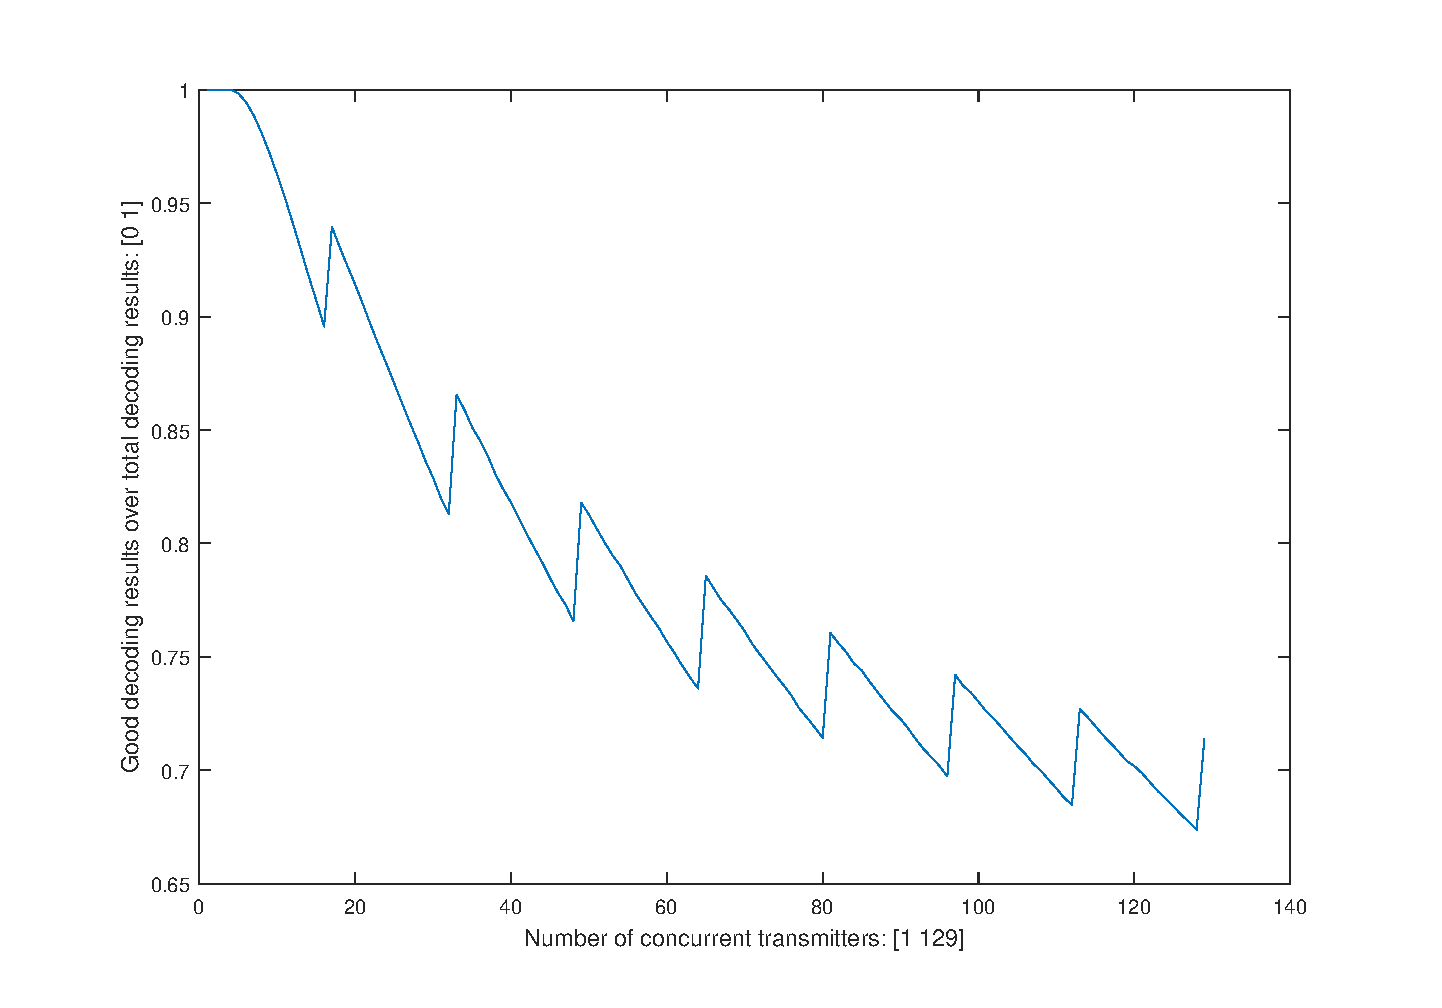
\includegraphics[width=\textwidth]{chapters/decoding-sim-gold-n7.eps}
			\caption{Decoding results when simulating with gold codes of length 127.}
			\label{fig:decoding-sim-gold-n7}
		\end{figure}

		\begin{equation}
			\label{eq:strange-peaks-distance-in-decoding-sim}
				\begin{cases}
					2^{\frac{n+1}{2}} & \quad \text{for odd } n \\
					2^{\frac{n+2}{2}} & \quad \text{for even } n \\
				\end{cases}
		\end{equation}

